\documentclass[10pt]{beamer}

\usetheme[progressbar=frametitle]{metropolis}
\usepackage{appendixnumberbeamer}
\usepackage{smartdiagram}
\usepackage{booktabs}
\usepackage[scale=2]{ccicons}
\usepackage{tabto}

\usepackage{pgfplots}
\usepgfplotslibrary{dateplot}

\usepackage{xspace}
\newcommand{\themename}{\textbf{\textsc{metropolis}}\xspace}

\title{Vershon control}
\subtitle{(using git)}
%\date{\today}
%\date{}
\author{\textbf{Danny Awty-Carroll}}
\institute{\tiny{\date{\today}}}
\titlegraphic{\hfill
\includegraphics[height=1cm]{Aberystwyth_University_logo}}


\begin{document}

\maketitle



\begin{frame}{Sections}
This will focus on using git in windows with a UI
\newline

  \setbeamertemplate{section in toc}[sections numbered]
  \tableofcontents[hideallsubsections]
\end{frame}




\section{Why version control?}


\begin{frame}[fragile]{What is version control}
This is just the manigment of vershons of a document.\\
One document through time.
  \begin{columns}[T]
    \begin{column}{.5\textwidth}
	
\includegraphics[width=6cm]{Figs/old/no}
    \end{column}
    \begin{column}{.5\textwidth}
	
\includegraphics[width=6cm]{Figs/old/date}
    \end{column}
  \end{columns}
All of us use some version control
\end{frame}


\begin{frame}[fragile]{Where things get complicated}
Numbering or dating documents works OK but can fall down when\\
	\begin{itemize}
		\item There are multiple documents that need to work together (i.e. a script and data)
		\item There are multiple people working on the documents (are they on the latist vertion and merging changes)
		\item There are updates to the progect that may brake things
		\item Line changes need to be reviewed
	\end{itemize}

Some of this is solved in programs like word with track changes (so you see who altered what when)
\end{frame}


\begin{frame}[fragile]{What version control systems can do}
	\begin{itemize}
		\item Give line by line user by user line changes
		\item Make a stucher to vershons so there can be side branches
		\item Minimise problems of multiple users working on the same document at the same time
	\end{itemize}
	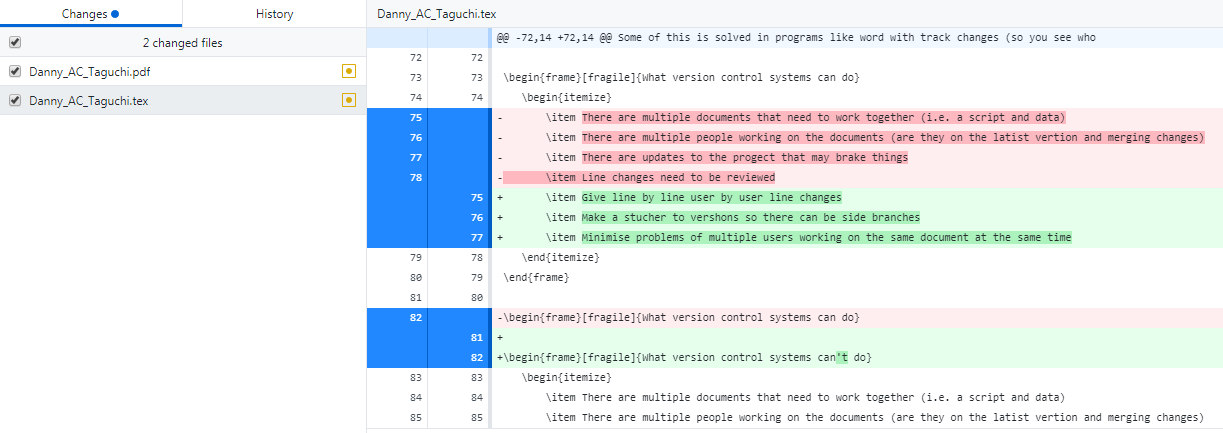
\includegraphics[width=11cm]{Figs/GHD/change}
\end{frame}


\begin{frame}[fragile]{What version control systems can't do}
	\begin{itemize}
		\item Add much extra control to binary files (not plan text)
		\item Back up in real time
	\end{itemize}
	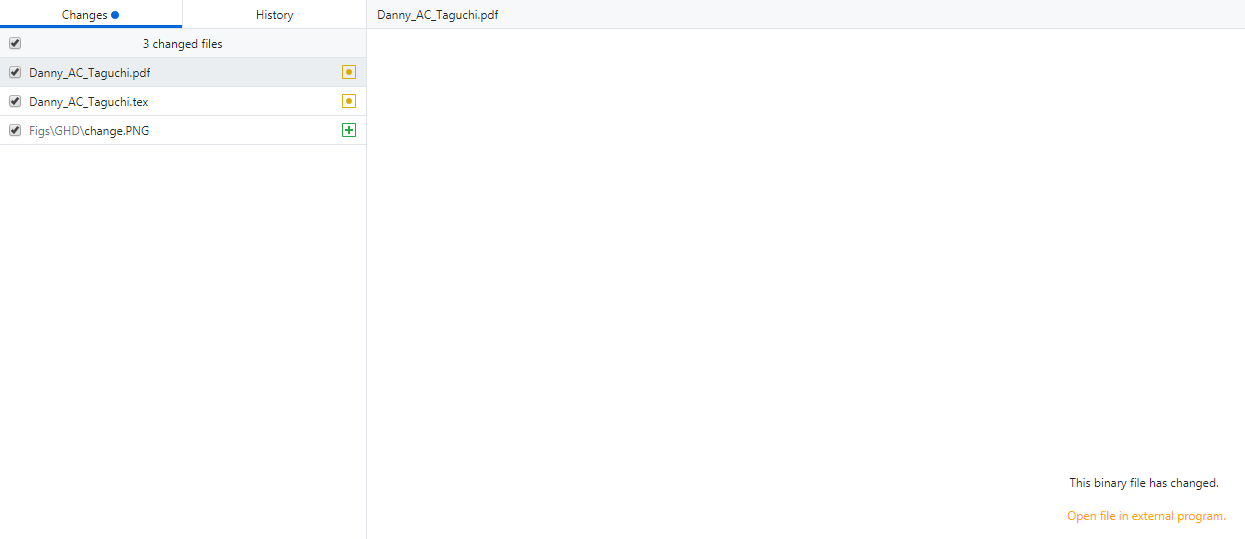
\includegraphics[width=11cm]{Figs/GHD/binarychange}
\end{frame}



\section{Version control system}


\begin{frame}[fragile]{What version control system?}
The first thing about version control systems is which system (we will cover git) \\
  \begin{columns}[T]
    \begin{column}{.8\textwidth}
	\smartdiagram[bubble diagram]{Effective\\ version\\ control,
 	System, Storage/\\platform, UI/\\interface}
    \end{column}
    \begin{column}{.2\textwidth}
	
\includegraphics[width=2cm]{Figs/Git-logo}
    \end{column}
  \end{columns}
\end{frame}


\begin{frame}[fragile]{What version control system?}
  \begin{columns}[T]
    \begin{column}{.8\textwidth}
	\begin{itemize}
		\item There are two populer version control systems (git  SVN)
		\item We will cover git as it is the most populer, the one I know and easyist to use
		\item Git was developed in 2005 by Linus Torvalds (Principal developer of Linux)
  		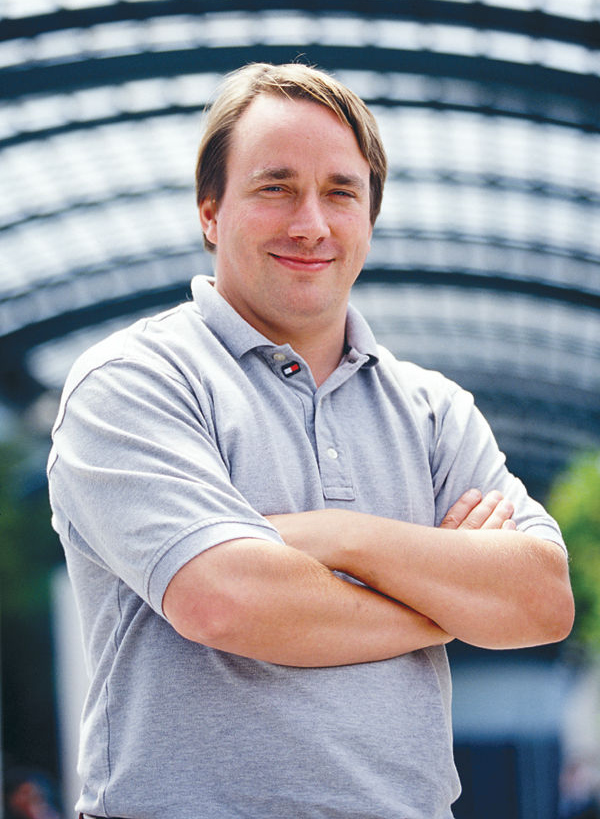
\includegraphics[width=2cm]{Figs/Linus_Torvalds}
	\end{itemize}
    \end{column}
    \begin{column}{.2\textwidth}
	
\includegraphics[width=2cm]{Figs/SVN} \newline \newline
	
\includegraphics[width=2cm]{Figs/Git-logo}
    \end{column}
  \end{columns}
\end{frame}


\begin{frame}[fragile]{What is git?}
  \begin{columns}[T]
    \begin{column}{.8\textwidth}
    \end{column}
    \begin{column}{.2\textwidth}
	
\includegraphics[width=2cm]{Figs/Git-logo}
    \end{column}
  \end{columns}
	\begin{itemize}
		\item Git is just system of version control
		\item By default it is used through a terminal
		\includegraphics[width=4cm]{Figs/git/status}
		\item Git has progects cauld reposetrys (or repos)
		\item It then has a tree struchure to manige the vershons
	\end{itemize}
\end{frame}


\begin{frame}[fragile]{Tree structure?}
  \begin{columns}[T]
    \begin{column}{.8\textwidth}
	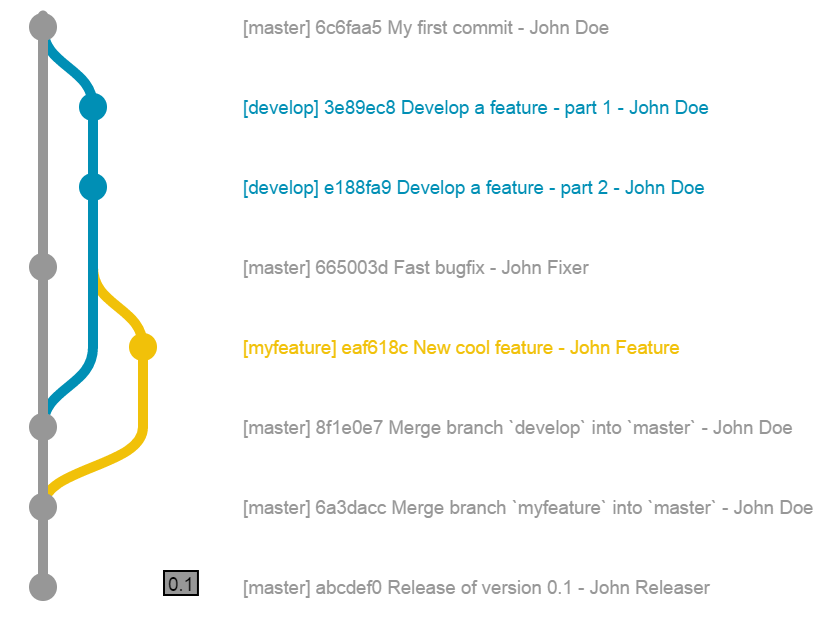
\includegraphics[width=9cm]{Figs/git/tree}
    \end{column}
    \begin{column}{.2\textwidth}
	
\includegraphics[width=2cm]{Figs/Git-logo} \newline  \newline
	The master branch is in gray with colour branches coming of and then being merged back
    \end{column}
  \end{columns}
\end{frame}


\begin{frame}[fragile]{Key comards?}
  \begin{columns}[T]
    \begin{column}{.8\textwidth}
	In the terminal interface there are some useful commards:
    \end{column}
    \begin{column}{.2\textwidth}
	
\includegraphics[width=2cm]{Figs/Git-logo}
    \end{column}
  \end{columns}
	\begin{itemize}
		\item \textit{init} - inisholies a repo
		\item \textit{status} - tells you if you have flies out of sync with the current vertion
		\item \textit{commit} - adds commits to the current vertion - a change with a comment and an ID
		\item \textit{add} - adds new files and current commit
		\item \textit{remove} - removes files and current commit
		\item \textit{push} - pushes comits to an online repo (only if using a git platform)
		\item \textit{pull} - pulls commits from an online platform (only if using a git platform)
	\end{itemize}
\end{frame}



\section{Platform}


\begin{frame}[fragile]{Which platform?}
You can just use git with the treminal on your PC or you can store work on an online reposetry mainging site, the most populer of these are GitHub and Bitbucket\\
  \begin{columns}[T]
    \begin{column}{.8\textwidth}
	\smartdiagram[bubble diagram]{Effective\\ version\\ control,
 	System, Storage/\\platform, UI/\\interface}
    \end{column}
    \begin{column}{.2\textwidth}
	
\includegraphics[width=2cm]{Figs/git/Octocat} \newline  \newline   \newline 
	
\includegraphics[width=2cm]{Figs/git/Bitbucket}
    \end{column}
  \end{columns}
\end{frame}


\begin{frame}[fragile]{Why not just store the repostry on dropbox?}
You can and it would be baked up and sherable, but there are problems:\\
  \begin{columns}[T]
    \begin{column}{.8\textwidth}
	\begin{itemize}
		\item You can run into Dropbox syncing and git version control clashes
		\item If you shere the files with a colaborator they are't identifyed separately to you
		\item You or a colaborator can completely mess up the git system (mostly by deleating the records in the `.git' folder)
		\item If you do you can't just re download
	\end{itemize}
    \end{column}
    \begin{column}{.2\textwidth}
	
\includegraphics[width=2cm]{Figs/git/Dropbox}
    \end{column}
  \end{columns}
\end{frame}


\begin{frame}[fragile]{Which platform?}
  \begin{columns}[T]
    \begin{column}{.8\textwidth}
	\textbf{Bitbucket}
	\begin{itemize}
		\item Alows unlimetd public or privet repostorys
		\item Charges per colcolaberaters over 5 on the repostorys 
		\item 1GB stroige for large flies all repostorys, 5GB if using a .ac email
	\end{itemize}
	\textbf{GitHub}
	\begin{itemize}
		\item Has unlimeted public repostorys 
		\item With unlimeted collaborators
		\item Pay for privet repostorys
		\item However as a student or academic you can sign up for free privet repostorys
		\item Github is about $\times$4 more populer than Bitbucket
	\end{itemize}
    \end{column}
    \begin{column}{.2\textwidth}
	
\includegraphics[width=2cm]{Figs/git/Bitbucket} \newline  \newline   \newline \newline 
	
\includegraphics[width=2cm]{Figs/git/Octocat}
    \end{column}
  \end{columns}
\end{frame}



\section{UI}


\begin{frame}[fragile]{Which UI?}
You can just use git with the treminal but there is a frendlyer interfase\\
  \begin{columns}[T]
    \begin{column}{.8\textwidth}
	\smartdiagram[bubble diagram]{Effective\\ version\\ control,
 	System, Storage/\\platform, UI/\\interface}
    \end{column}
    \begin{column}{.2\textwidth}
	
\includegraphics[width=2cm]{Figs/git/terminal} \newline  \newline   \newline 
	
\includegraphics[width=2cm]{Figs/git/gitdesktop} \newline  \newline   \newline 
	
\includegraphics[width=2cm]{Figs/git/Sourcetree}
    \end{column}
  \end{columns}
\end{frame}


\begin{frame}[fragile]{Which UI?}
  \begin{columns}[T]
    \begin{column}{.8\textwidth}
  	\textbf{The Terminal\\}
	You can just use the termainal with the raw git commands as seen before... but:
	\begin{itemize}
		\item If you are not using it enyway or are happy using it a graphical UI is nice 
		\item You don't need to remember commands or reposty names 
	\end{itemize}
	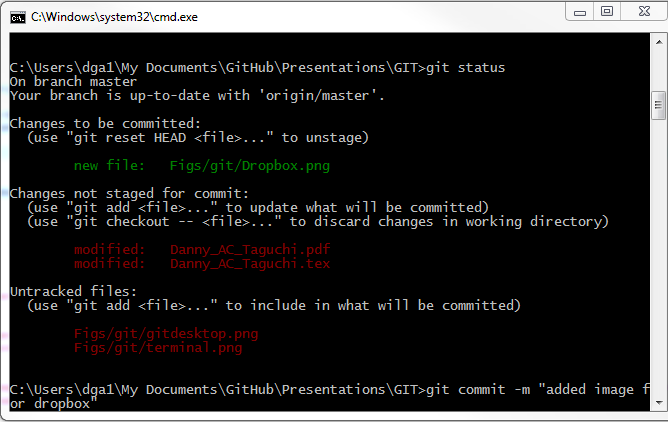
\includegraphics[width=6cm]{Figs/git/terminaluse}
    \end{column}
    \begin{column}{.2\textwidth}
	
\includegraphics[width=2cm]{Figs/git/terminal} \newline  \newline  \newline 
    \end{column}
  \end{columns}
\end{frame}



\begin{frame}[fragile]{Which UI?}
  \begin{columns}[T]
    \begin{column}{.8\textwidth}
  	\textbf{Git Desktop\\}
	The easyist to use and most populer UI is git desktop:
	\begin{itemize}
		\item This is made by github and intigrates very well with github or local (on pc) reposotrys
		\item It will work with other hosting platforms but less easly
		\item Is the easyist to use
	\end{itemize}
	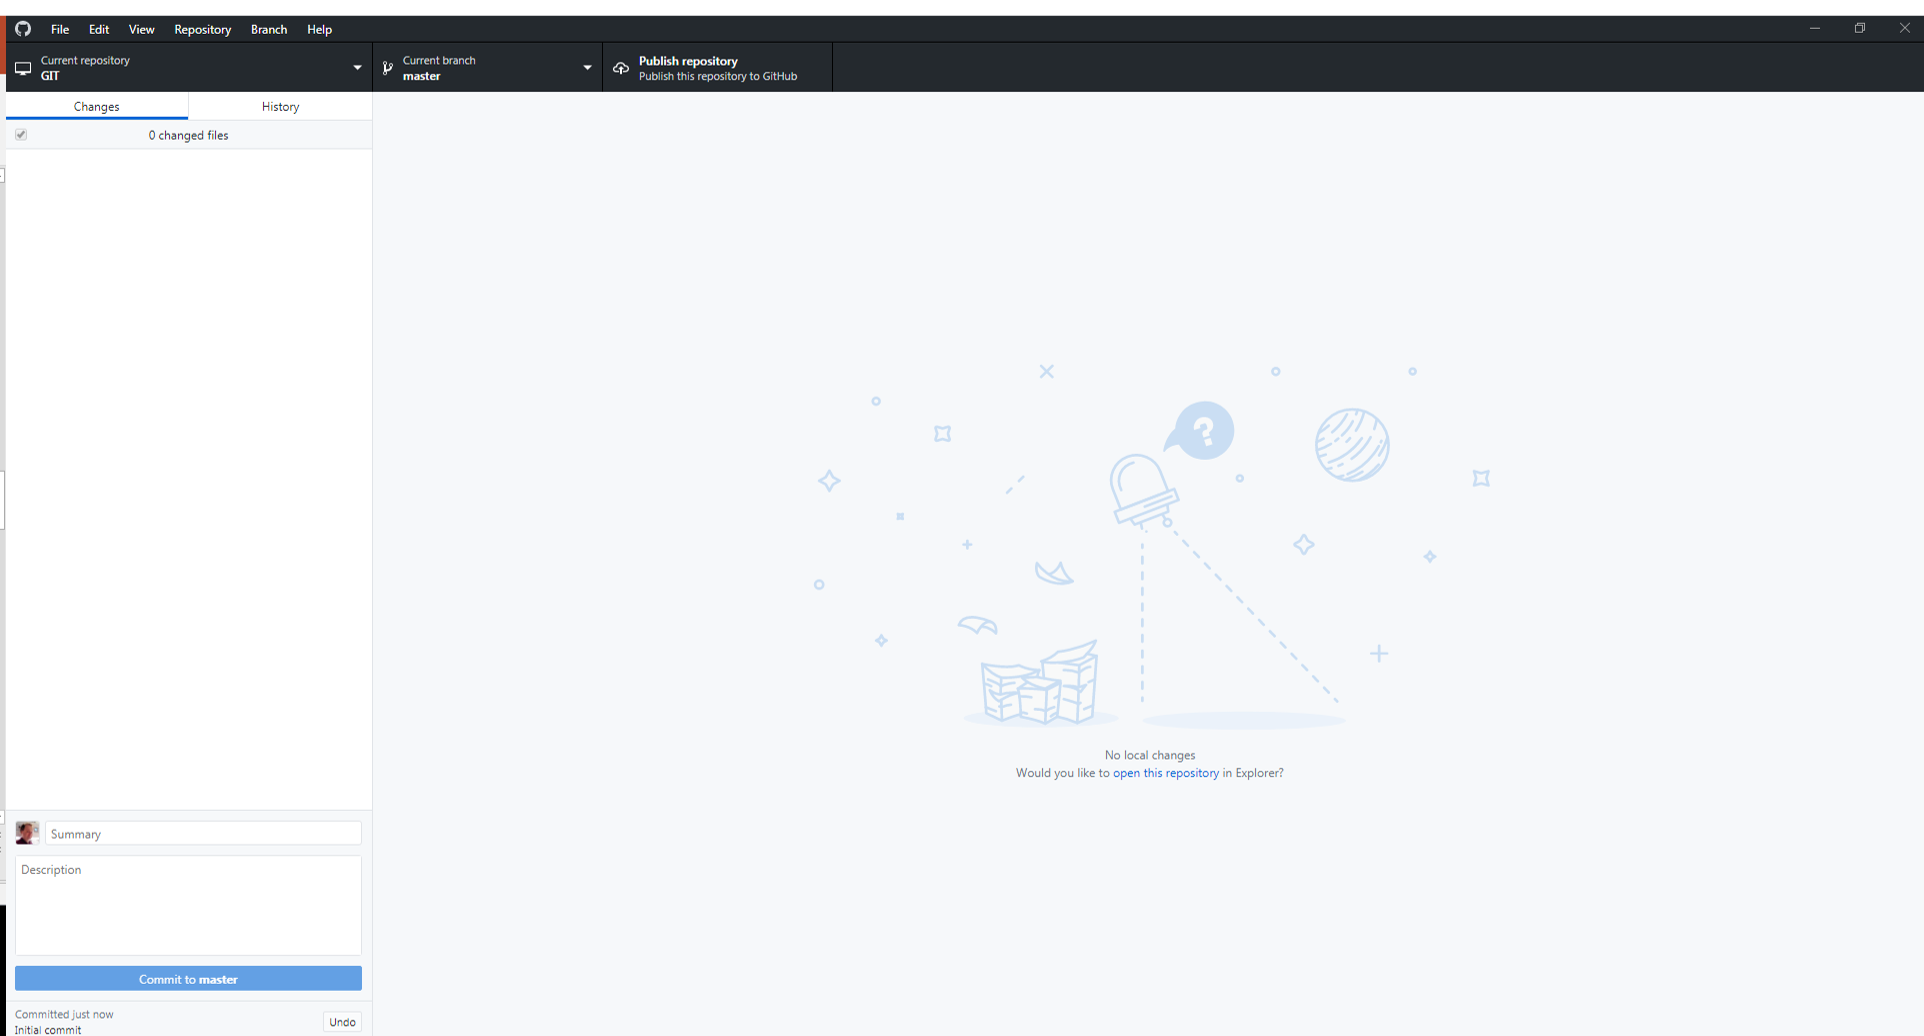
\includegraphics[width=8cm]{Figs/GHD/outline_02}
    \end{column}
    \begin{column}{.2\textwidth}
	
\includegraphics[width=2cm]{Figs/git/gitdesktop} \newline  \newline  \newline 
    \end{column}
  \end{columns}
\end{frame}


\begin{frame}[fragile]{Which UI?}
  \begin{columns}[T]
    \begin{column}{.8\textwidth}
  	\textbf{Sourcetree\\}
	The hosting platform indipendet :
	\begin{itemize}
		\item Sourcetree is uned by atlassian who ouns Bitbucket
		\item It will work with other hosting platforms easly
	\end{itemize}
	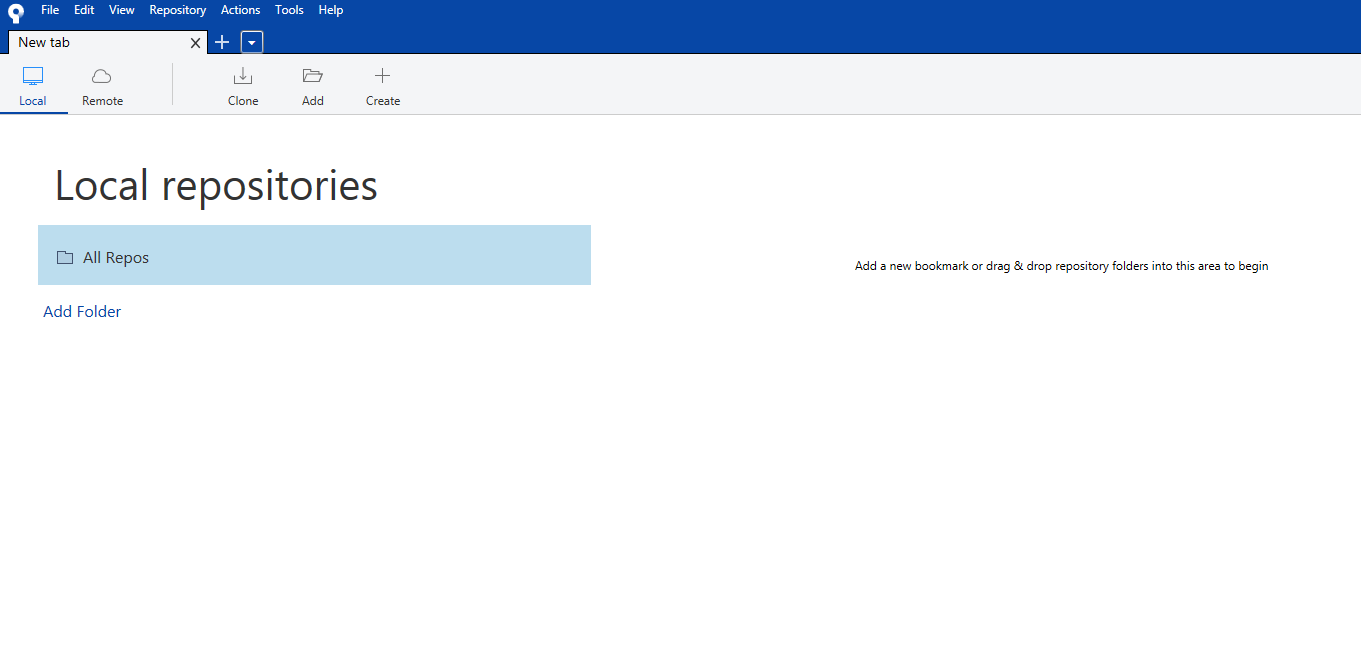
\includegraphics[width=8cm]{Figs/ST/ST_00}
    \end{column}
    \begin{column}{.2\textwidth}
	
\includegraphics[width=2cm]{Figs/git/Sourcetree} \newline  \newline  \newline 
    \end{column}
  \end{columns}
\end{frame}





%\begin{frame}[fragile]{Used\dots}
%Taguchi design is based on performing experiments with complex combinations of factors then calculating the signal to noise in the results from the factors.
%	
%	\begin{itemize}
%		\item Each factor is replicated independently of other factors
%		\item So a small number of experiments can show possible differences for many factors
%	\end{itemize}
%
%e.g. With a traditional factorial experimental design investigating $4$ factors with $3$ levels and $3$ replicates would require $36$ experimental units, un-replicated this would still require $12$. The Taguchi DOE would only require $9$ experimental units.
%\end{frame}
%
%
%{%
%\setbeamertemplate{frame footer}{\cite{roy2001design, roy2010primer, SubbaRao2008}}
%\begin{frame}{OEC}
%The Taguchi can also apply a summary statistic as an Overall Evaluation Criteria (OEC) \\ \vspace{4mm}
%The OEC can then determine which set of treatments were the best for seedlings based on all of the experimental responses
%\begin{exampleblock}{ }
%\[
%OEC =\left( \frac{y_1}{y_{1\,max}} \right) \cdot w_1 + \left( \frac{y_2}{y_{2\,max}} \right) \cdot w_2 + \dots
%\]
%\end{exampleblock}
%Where $y_i$ is the response measurement, $y_{i\,max}$ is the maximum value for the response, and $w_i$ is the weighing of the response.
%\end{frame}
%}
%
%
%{%
%\setbeamertemplate{frame footer}{\cite{Yaldagard2008, rao2008taguchi}}
%\begin{frame}[fragile]{Why germination}
%Successful germination of \textit{\textit{Miscanthus}} seed is vital for the commercial uptake of new \textit{Miscanthus} hybrids.
%	\begin{itemize}
%		\item Germination can be affected by a large number of stresses and hormones that can interact
%		\item These factors can easily have differing effects at high levels
%		\item Taguchi has been used in to test priming in barley
%		\item But usage is still novel in the biological sciences
%	\end{itemize}
%These things make germination an interesting test for the Taguchi DOE
%\end{frame}
%}
%
%
%
%\section{Parametrising germination}
%
%
%
%\begin{frame}{Parametrising}
%		To parametrise the Taguchi things that could be tested together were 
%chosen so as many variables as possible could be kept the same \\ \vspace{10mm}
%  \begin{columns}[T]
%    \begin{column}{.5\textwidth}
%    	\centering{To test}
%        \begin{itemize}
%            \item Water soluble hormones
%            \item Water stress
%            \item Lighting
%            \item Priming
%        \end{itemize}
%    \end{column}
%    \begin{column}{.5\textwidth}
%    	\centering{To maintain}
%        \begin{itemize}
%            \item Syn55 \textit{M. sinensis} seed
%            \item Dish setup
%            \item Experimental run time
%            \item What to record
%        \end{itemize}
%    \end{column}
%  \end{columns}
%  \vspace{10mm}
%  This allows the parametrisation experiments to inform the Taguchi
%\end{frame}
%
%
%\begin{frame}{Selecting variables}
%	Things that could be tested together were chosen \textit{- excluding gasses etc.}
%        \begin{columns}[T]
%    	\begin{column}{.1\textwidth}
%        
%    	\end{column}
%    	\begin{column}{.9\textwidth}
%          \begin{itemize}
%              \item \alert<+>{Abscisic acid} \footnotesize \tabto{3.5cm} \color{lightgray} \only<1>{\color{black}}[0.05 to 60 (mg L$^{-1}$)] \normalsize \color{black}
%              \item \alert<+>{Gibberellic acid} \footnotesize \tabto{3.5cm} \color{lightgray} \only<2>{\color{black}}[0.15 to 750 (mg L$^{-1}$)] \normalsize \color{black}
%              \item \alert<+>{Auxin} \footnotesize \tabto{3.5cm} \color{lightgray} \only<3>{\color{black}}[NAA 0.01 to 200 (mg L$^{-1}$)]  \normalsize \color{black}
%              \item \alert<+>{Brassinosteroid} \footnotesize \tabto{3.5cm} \color{lightgray} \only<4>{\color{black}}[0.001 to 2 (mg L$^{-1}$)] \normalsize \color{black}
%              \item \alert<+>{Water stress} \footnotesize \tabto{3.5cm} \color{lightgray} \only<5>{\color{black}}[PEG 4000 \& 8000 0.05 to 4.1 (-MPa)] \normalsize \color{black}
%              \item \alert<+>{Salinity} \footnotesize \tabto{3.5cm} \color{lightgray} \only<6>{\color{black}}[0.05 to 4.1 (-MPa)] \normalsize \color{black}
%              \item \alert<+>{Light levels} \footnotesize \tabto{3.5cm} \color{lightgray} \only<7>{\color{black}}[light vs no light] \normalsize \color{black}
%              \item \alert<+>{Seed priming} \footnotesize \tabto{3.5cm} \color{lightgray} \only<8>{\color{black}}[Water priming] \normalsize \color{black}
%          \end{itemize}
%    	\end{column}
%  \end{columns}
%    \vspace{10mm}
%    Using a wide range for the selected variables
%\end{frame}
%
%
%\begin{frame}{Setup}
%	All but the light experiments were setup in the same way to produce consistent results
%    \begin{columns}[T]
%    	\begin{column}{.5\textwidth}
%			\begin{itemize}[<+->]
%                \pause
%				\item 64 seeds on a Petri dish per treatment
%                \item Germination was scored daily for 11 days
%                \item The hormone, salt or PEG was diluted into the water used to wet the dish.
%			\end{itemize}
%    	\end{column}
%    	\begin{column}{.5\textwidth}
%			\includegraphics[width=6cm]{Figs/Dish}
%    	\end{column}
%  \end{columns}
%\end{frame}
%
%
%
%\section{Results}
%
%
%
%\begin{frame}{Abscisic Acid}
%  \begin{columns}[T]
%    \begin{column}{.5\textwidth}
%	\includegraphics[width=6cm]{Figs/ABA/StemRoot}
%    \end{column}
%    \begin{column}{.5\textwidth}
%	\includegraphics[width=6cm]{Figs/ABA/GermTime}
%    \end{column}
%  \end{columns}
%\end{frame}
%
%
%\begin{frame}{Gibberellic Acid}
%  \begin{columns}[T]
%    \begin{column}{.5\textwidth}
%	\includegraphics[width=6cm]{Figs/GA/StemRoot}
%    \end{column}
%    \begin{column}{.5\textwidth}
%	\includegraphics[width=6cm]{Figs/GA/GermTime}
%    \end{column}
%  \end{columns}
%\end{frame}
%
%
%\begin{frame}{Auxin}
%  \begin{columns}[T]
%    \begin{column}{.5\textwidth}
%	\includegraphics[width=6cm]{Figs/NAA/StemRoot}
%    \end{column}
%    \begin{column}{.5\textwidth}
%	\includegraphics[width=6cm]{Figs/NAA/GermTime}
%    \end{column}
%  \end{columns}
%\end{frame}
%
%
%\begin{frame}{Brassinosteroid}
%  \begin{columns}[T]
%    \begin{column}{.5\textwidth}
%	\includegraphics[width=6cm]{Figs/BR/StemRoot}
%    \end{column}
%    \begin{column}{.5\textwidth}
%	\includegraphics[width=6cm]{Figs/BR/GermTime}
%    \end{column}
%  \end{columns}
%\end{frame}
%
%
%\begin{frame}{Water Stress}
%  \begin{columns}[T]
%    \begin{column}{.5\textwidth}
%	\includegraphics[width=6cm]{Figs/PEG/StemRoot}
%    \end{column}
%    \begin{column}{.5\textwidth}
%	\includegraphics[width=6cm]{Figs/PEG/GermTime}
%    \end{column}
%  \end{columns}
%\end{frame}
%
%
%\begin{frame}{Salinity}
%  \begin{columns}[T]
%    \begin{column}{.5\textwidth}
%	\includegraphics[width=6cm]{Figs/NaCl/StemRoot}
%    \end{column}
%    \begin{column}{.5\textwidth}
%	\includegraphics[width=6cm]{Figs/NaCl/GermTime}
%    \end{column}
%  \end{columns}
%\end{frame}
%
%
%\begin{frame}{Light}
%  \begin{columns}[T]
%    \begin{column}{.5\textwidth}
%		Syn55 \textit{M. sinensis}\\ \vspace{5mm}
%		Germinated and grown in the dark \\ \vspace{5mm}
%		There was no significant difference in germination\\ \vspace{5mm}
%		Seedlings dry weights taken after 1 month\\ \vspace{5mm}
%		There is an indication of boost in dry weight after a short exposure to dark
%    \end{column}
%    \begin{column}{.5\textwidth}
%	\includegraphics[width=6cm]{Figs/Light/DB}
%    \end{column}
%  \end{columns}
%\end{frame}
%
%
%\begin{frame}{Light}
%  \begin{columns}[T]
%    \begin{column}{.5\textwidth}
%	\includegraphics[width=6cm]{Figs/Light/GermP}
%    \end{column}
%    \begin{column}{.5\textwidth}
%		Try four genotypes for dark germination \\ \vspace{5mm}
%		MX300 and Syn55 are \textit{M. sinensis}\\ \vspace{5mm}
%		GNT14 is a \textit{lutarioriparius $\times$ sinensis} hybrid\\ \vspace{5mm}
%		Syn70 is a \textit{M. sacchariflorus}
%    \end{column}
%  \end{columns}
%\end{frame}
%
%
%{%
%\setbeamertemplate{frame footer}{Technologica Ltd (Colchester, UK)}
%\begin{frame}{Priming}
%  \begin{columns}[T]
%    \begin{column}{.5\textwidth}
%      \includegraphics[width=6cm]{Figs/Prime/Flo}
%      \vspace{2mm}
%      \small{Chlorophyll fluorescence done using the CF Imager}
%    \end{column}
%    \begin{column}{.5\textwidth}
%      	Priming made no significant differences to germination \\ \vspace{5mm}
%      	Produced some negative effects in laboratory testing\\ \vspace{5mm}
%        e.g. Area of chlorophyll fluorescence for 100 seeds over time \\ \vspace{5mm}
%    \end{column}
%  \end{columns}
%\end{frame}
%}
%
%
%
%\section{Taguchi set-up}
%
%
%
%\begin{frame}{Taguchi Set-up}
%	Things that could be tested together were chosen.\newline
%	levels were selected based on an appropriately sized Taguchi Grid.
%	\begin{itemize}
%	\item Two level designs can be  L$_{4}$, L$_{8}$,  L$_{12}$ or L$_{16}$
%	\item Three level designs can be  L$_{9}$ and L$_{27}$
%	\item There are also mixed factor designs that are L$_{8}$, L$_{16}$ and L$_{18}$ these allow different numbers of factors per variable. 
%	\end{itemize}
%\pause
%e.g L$_4$ 
%\begin{table}[htpb]\scriptsize
%\centering
%\begin{tabular}{p{2cm} |  p{1cm}   p{1cm}  p{1cm}}
%\hline
%\textbf{Experiment N\textsuperscript{\underline{o}}} & \textbf{A}   & \textbf{B}  & \textbf{C}  \\
%\hline
%1 & High  & High & High\\
%2 & High  & Low & Low\\
%3 & Low  & High & Low\\
%4 & Low  & Low & High\\
%\hline
%\end{tabular}
%\end{table}
%\end{frame}
%
%
%\begin{frame}{Selecting the Taguchi}
%	A L$_{16}$ mixed level Taguchi Design was chosen, to allow four factors at four levels and three factors at two levels.
%\begin{table}[htpb]\scriptsize
%\centering
%\begin{tabular}{p{1cm} |  p{1cm}   p{1cm}  p{1cm}   p{1cm}  p{1cm}   p{1cm} p{1cm}   p{1cm}}
%\hline
%\textbf{Experi- ment N\textsuperscript{\underline{o}}} & \textbf{ABA  $(mg\, l^{-1})$}   & \textbf{GA  $(mg\, l^{-1})$}  & \textbf{Water Stress  $(Mpa)$}  & \textbf{NAA  $(mg\, l^{-1})$}  & \textbf{BR  $(mg\, l^{-1})$} & \textbf{Light Level} & \textbf{Primed Seeds}\\
%\hline
%1 & V-Low  & V-Low & Low & V-Low  & V-Low & Low & Yes\\
%2 & V-Low  & Low & Low & Low  & Low & High & No\\
%3 & V-Low  & High & High & High  & High & Low & No\\
%4 & V-Low  & V-High & High & V-High  & V-High & High & Yes\\
%5 & Low  & V-Low & Low & V-High  & High & High & No\\
%6 & Low  & Low & Low & High  & V-High & Low & Yes\\
%7 & Low  & High & High & Low  & V-Low & High & Yes\\
%8 & Low  & V-High & High & V-Low  & Low & Low & No\\
%9 & High  & V-Low & High & Low  & V-High & Low & No\\
%10 & High  & Low & High & V-Low  & High & High & Yes\\
%11 & High  & High & Low & V-High  & Low & Low & Yes\\
%12 & High  & V-High & Low & High  & V-Low & High & No\\
%13 & V-High  & V-Low & High & High  & Low & High & Yes\\
%14 & V-High  & Low & High & V-High  & V-Low & Low & No\\
%15 & V-High  & High & Low & V-Low  & V-High & High & No\\
%16 & V-High  & V-High & Low & Low  & High & Low & Yes\\
%\hline
%\end{tabular}
%\end{table}
%\end{frame}
%
%
%\begin{frame}[fragile]{OEC}
%  OEC weightings were subjective but were selected on the principle of a higher weighting for a broader output \\ \vspace{2mm}
%  So GI was weighted highest at $25\%$, because it represents germination speed and quantity \\ \vspace{2mm}
%  The stem:root ratio was second, weighted at $20\%$ because it gives an indication of the overall health of the seedlings growth \\ \vspace{2mm}
%  Both Fv/Fm fluorescence measures at $15\%$ \\ \vspace{2mm}
%  Germination percentage and 1/T$_{50}$ weighted at $7.5\%$ \\ \vspace{2mm}
%  Root and stem elongation were weighted at $5\%$ \\ \vspace{2mm}
%\end{frame}
%
%
%\begin{frame}{Paramitrising}
%	These levels needed filling in dependent on the range finding experiments.   \newline
%   	\begin{itemize}[<+->]
%                \pause
%	      \item[] Abscisic Acid  levels of 0.02, 0.2, 2, and 20 mg L$^{-1}$
%                \item[] Gibberellic Acid levels of  0.015, 0.15, 1.5, and 15 mg L$^{-1}$ 
%                \item[] Auxin levels of 0.005, 0.05, 0.5, and 5 mg  L$^{-1}$
%                \item[] PEG induced $\Psi$ stress of -0.01  and -0.5 MPa 
%                \item[] Brassinosteroid levels of 0.015, 0.75, 1.5, and 7.5 mg  L$^{-1}$
%                \item[] Light levels of 300 to 80 μmol m$^{-2}$ s$^{-1}$ 
%                \item[] Water primed and non water primed Syn55 seed
%	\end{itemize}
%\end{frame}
%
%
%
%\section{Taguchi results}
%
%
%
%\begin{frame}{Raw output}
%	This is the output of the experiments\dots
%\begin{table}[htpb]\scriptsize
%\centering
%\begin{tabular}{p{1.2cm} |  p{1cm}   p{0.5cm}  p{0.8cm}   p{0.8cm}  p{1cm}   p{0.8cm}  p{0.8cm}   p{0.8cm}}
%\hline
%\textbf{Experiment N\textsuperscript{\underline{o}}} & \textbf{Germ- ination Index}   & \textbf{Stem: Root}  & \textbf{Fv/Fm Area}  & \textbf{Fv/Fm Median}  & \textbf{Percentage Germ 7d} & \textbf{Germ Rate $(1/T_{50})$} & \textbf{Stem Elongation} & \textbf{Root Elongation}\\
%\hline
%1   &      1.69    &    3.64   &    	338.6   &    	0.796   &    	29.7   &    	0.031   &    	12.21   &    	3.35\\
%2   &      3.05    &    2.52   &    	375.4   &    	0.739   &    	54.7   &    	0.029   &    	8.14   &    	3.24\\	
%3   &      2.34    &    1.96   &    	133.0   &    	0.776   &    	39.1   &   	0.036   &    	5.87   &    	3.00\\
%4   &      0.56    &    2.73   &    	32.4   &    	0.683   &    	12.5   &   	0.019   &    	5.00   &    	1.83\\
%5   &      2.48    &    2.69   &    	227.3   &    	0.774   &    	46.9   &   	0.024   &    	6.14   &    	2.29\\
%6   &      2.34    &    3.81   &    	345.6   &    	0.797   &    	40.6   &   	0.031   &    	11.08   &    	2.91\\ 
%7   &      0.42    &    1.40   &   	6.2   &    	0.271   &    	7.8   &   	0.027   &    	1.40   &    	1.00\\
%8   &      2.83    &    1.79   &    	207.0   &    	0.764   &    	48.4   &    	0.033   &    	6.45   &    	3.61\\ 
%9   &      2.28    &    1.04   &    	10.0   &    	0.68   &    	39.1   &   	0.032   &    	1.36   &    	1.31\\
%10   &    0.27   &     1.00   &    	0.5   &    	0.261   &    	4.7   &    	0.028   &    	1.00   &    	1.00\\
%11   &    2.09   &     2.94   &    	225.0   &    	0.775   &    	34.4   &    	0.043   &    	9.65   &    	3.28\\
%12   &    2.59   &     2.54   &    	161.8   &    	0.694   &   	46.9   &   	0.030   &    	6.50   &    	2.56\\
%13   &    0.27   &     1.00   &    	1.0   &    	0.201   &    	4.7   &    	0.031   &    	1.00   &    	1.00\\
%14   &    1.19   &     0.88   &    	10.9   &    	0.443   &    	21.9   &    	0.027   &    	1.46   &    	1.67\\
%15   &    2.17   &     1.05   &    	60.1   &    	0.735   &    	39.1   &    	0.027   &    	2.85   &    	2.70\\
%16   &    2.67   &     1.51   &    	55.7   &    	0.744   &    	46.9   &   	0.031   &    	2.52   &    	1.67\\
%\color{lightgray} Weighting & \color{lightgray} 0.25  & \color{lightgray} 0.2 & 	\color{lightgray} 0.15 & 	\color{lightgray} 0.15  & 	\color{lightgray} 0.075 & 	\color{lightgray} 0.075 &  	\color{lightgray} 0.05 & 	\color{lightgray} 0.05\\ 
%\hline
%\end{tabular}
%\end{table}
%\end{frame}
%
%
%
%\begin{frame}{Calculated effects}
%  \begin{columns}[T]
%    \begin{column}{8cm}
%	\includegraphics[width=8cm]{Figs/Taguchi_Pers_effects}
%    \end{column}
%    \begin{column}{4cm}
%	\vspace*{1.8cm}
%	The effect on each result by each input factor used. There is large effect of water stress and abscisic asid.\\ \vspace{5mm}
%	This does not specify if any affect is positive or negative. 
%    \end{column}
%  \end{columns}
%\end{frame}
%
%
%\begin{frame}{Best Levels}
%	The optimum level for each factor for each result
%	\includegraphics[width=8.5cm]{Figs/Tag_Best}
%\end{frame}
%
%
%\begin{frame}{OEC}
%  \begin{table}[htpb]\scriptsize
%  \centering
%  \begin{tabular}{p{1cm}  p{1cm}   p{1cm}  p{1cm}   p{1cm}  p{1cm}   p{1cm} | p{0.8cm} }
%  \hline
%  \textbf{ABA  $(mg\, l^{-1})$}   & \textbf{GA  $(mg\, l^{-1})$}  & \textbf{Water Stress  $(Mpa)$}  & \textbf{NAA  $(mg\, l^{-1})$}  & \textbf{BR  $(mg\, l^{-1})$} & \textbf{Light Level} & \textbf{Primed Seeds} & \textbf{OEC}\\
%  \hline
%  Low   &    Low   &    Low   &    High   &    V-High   &    Low   &    Yes   &    84.886\\
%  V-Low   &    Low   &    Low   &    Low   &    Low   &    High   &    No   &    83.049\\
%  V-Low   &    V-Low   &    Low   &    V-Low   &    V-Low   &    Low   &    Yes   &    77.302\\
%  High   &    High   &    Low   &    V-High   &    Low   &    Low   &    Yes   &    74.090\\
%  Low   &    V-High   &    High   &    V-Low   &    Low   &    Low   &    No   &    70.203\\
%  Low   &    V-Low   &    Low   &    V-High   &    High   &    High   &    No   &    68.634\\
%  High   &    V-High   &    Low   &    High   &    V-Low   &    High   &    No   &    66.477\\
%  V-Low   &    High   &    High   &    High   &    High   &    Low   &    No   &    62.291\\
%  V-High   &    V-High   &    Low   &    Low   &    High   &    Low   &    Yes   &    54.014\\
%  V-High   &    High   &    Low   &    V-Low   &    V-High   &    High   &    No   &    46.004\\
%  High   &    V-Low   &    High   &    Low   &    V-High   &    Low   &    No   &    41.693\\
%  V-Low   &    V-High   &    High   &    V-High   &    V-High   &    High   &    Yes   &    33.249\\
%  V-High   &    Low   &    High   &    V-High   &    V-Low   &    Low   &    No   &    21.395\\
%  Low   &    High   &    High   &    Low   &    V-Low   &    High   &    Yes   &    10.220\\
%  High   &    Low   &    High   &    V-Low   &    High   &    High   &    Yes   &    5.296\\
%  V-High	 & 	V-Low&	High&		High&		Low&		High&		Yes&		4.594\\
%  \hline
%  \end{tabular}
%  \end{table}
%  	Ordered by the OEC value
%\end{frame}
%
%
%\begin{frame}{Results Summary}
%	The best setup as identified by the OEC
%	\begin{table}[htpb]\small
%	\centering
%	\begin{tabular}{p{2.7cm} |  p{1.8cm}   p{1.8cm} }
%	\hline
%	\textbf{Factor}   & \textbf{Percentage Effect OEC}  & \textbf{Optimal Level OEC}\\
%	\hline
%	Abscisic Acid  &  21.2  &  V-Low\\
%	Gibberellic Acid  &  1.5  &  V-High\\	
%	Auxin  &  1  &  High\\
%	Brassinosteroid  &  3.8  &  Low\\
%	Water Stress  &  50.1  &  Low\\	
%	Light  &  15.2  &  Low\\
%	Priming  &   	7.2	   &  No \\
%	\hline
%	\end{tabular}
%	\end{table}
%    \vspace{4mm}
%    However, the larger table (previous) can be used to check the best outcome in a given scenario e.g. water stress
%\end{frame}



\section{Conclusions}

%\begin{frame}{Conclusions}
%Stem to root ratio was most affected from water stress, which is understandable because this may force the plant to change the deployment of resources between above and below ground. ABA also had a large effect, which is expected as a growth hormone. Whilst not a large effect, it was the measurement most effect by auxin, which again as a growth hormone it is not surprising that it changed the ratio of root to stem. It seems counter intuitive but lower light levels had a beneficial effect on all seed measurements; however, this was not zero light as in the preliminary experiments, here high light levels could have increased the evaporation rate and led to an interaction with water stress, this may need more investigation to resolve. It is unsurprising that plants with low water stress performed better in all measures. Water stress had an important effect on outcomes particularly in the health and growth measurements. ABA effect the most measurements.
%\end{frame}


{%
\setbeamertemplate{frame footer}{(xkcd)}
{\setbeamercolor{palette primary}{fg=gray, bg=gray}
\begin{frame}[standout]
  
\includegraphics[width=6.5cm]{Figs/xkcd}
\end{frame}
}


\appendix

%\begin{frame}[fragile]{Backup slides}
%  Sometimes, it is useful to add slides at the end of your presentation to
%  refer to during audience questions.

%  The best way to do this is to include the \verb|appendixnumberbeamer|
%  package in your preamble and call \verb|\appendix| before your backup slides.

%  \themename will automatically turn off slide numbering and progress bars for
%  slides in the appendix.
%\end{frame}

\begin{frame}[allowframebreaks]{References}

  \bibliography{Mendeley}
  \bibliographystyle{apalike}

\end{frame}

\end{document}
